\chapter{JT60-SA control design}

\section{Machine description}

JT60-SA is an under-construction superconductive tokamak located at one of the facilities from the National Institutes for Quantum and Radiological Science and Technology (QST)  at  Naka, Japan whose principal purpose is  the contribution to early realization of fusion energy by supporting the exploitation and resolving key physics for ITER reactor. Figure ~\ref{JT60schm} shows the overall general configuration and the most remarkable elements of the machine. The JT-60SA  vacuum chamber will have a major radius of 2.96 m and a minor radius of 1.18 m with an overall plasma volume of 132 $m^3$ ~\cite{Spears2014} .
\smallskip

\begin{figure}[h]
	\centering
	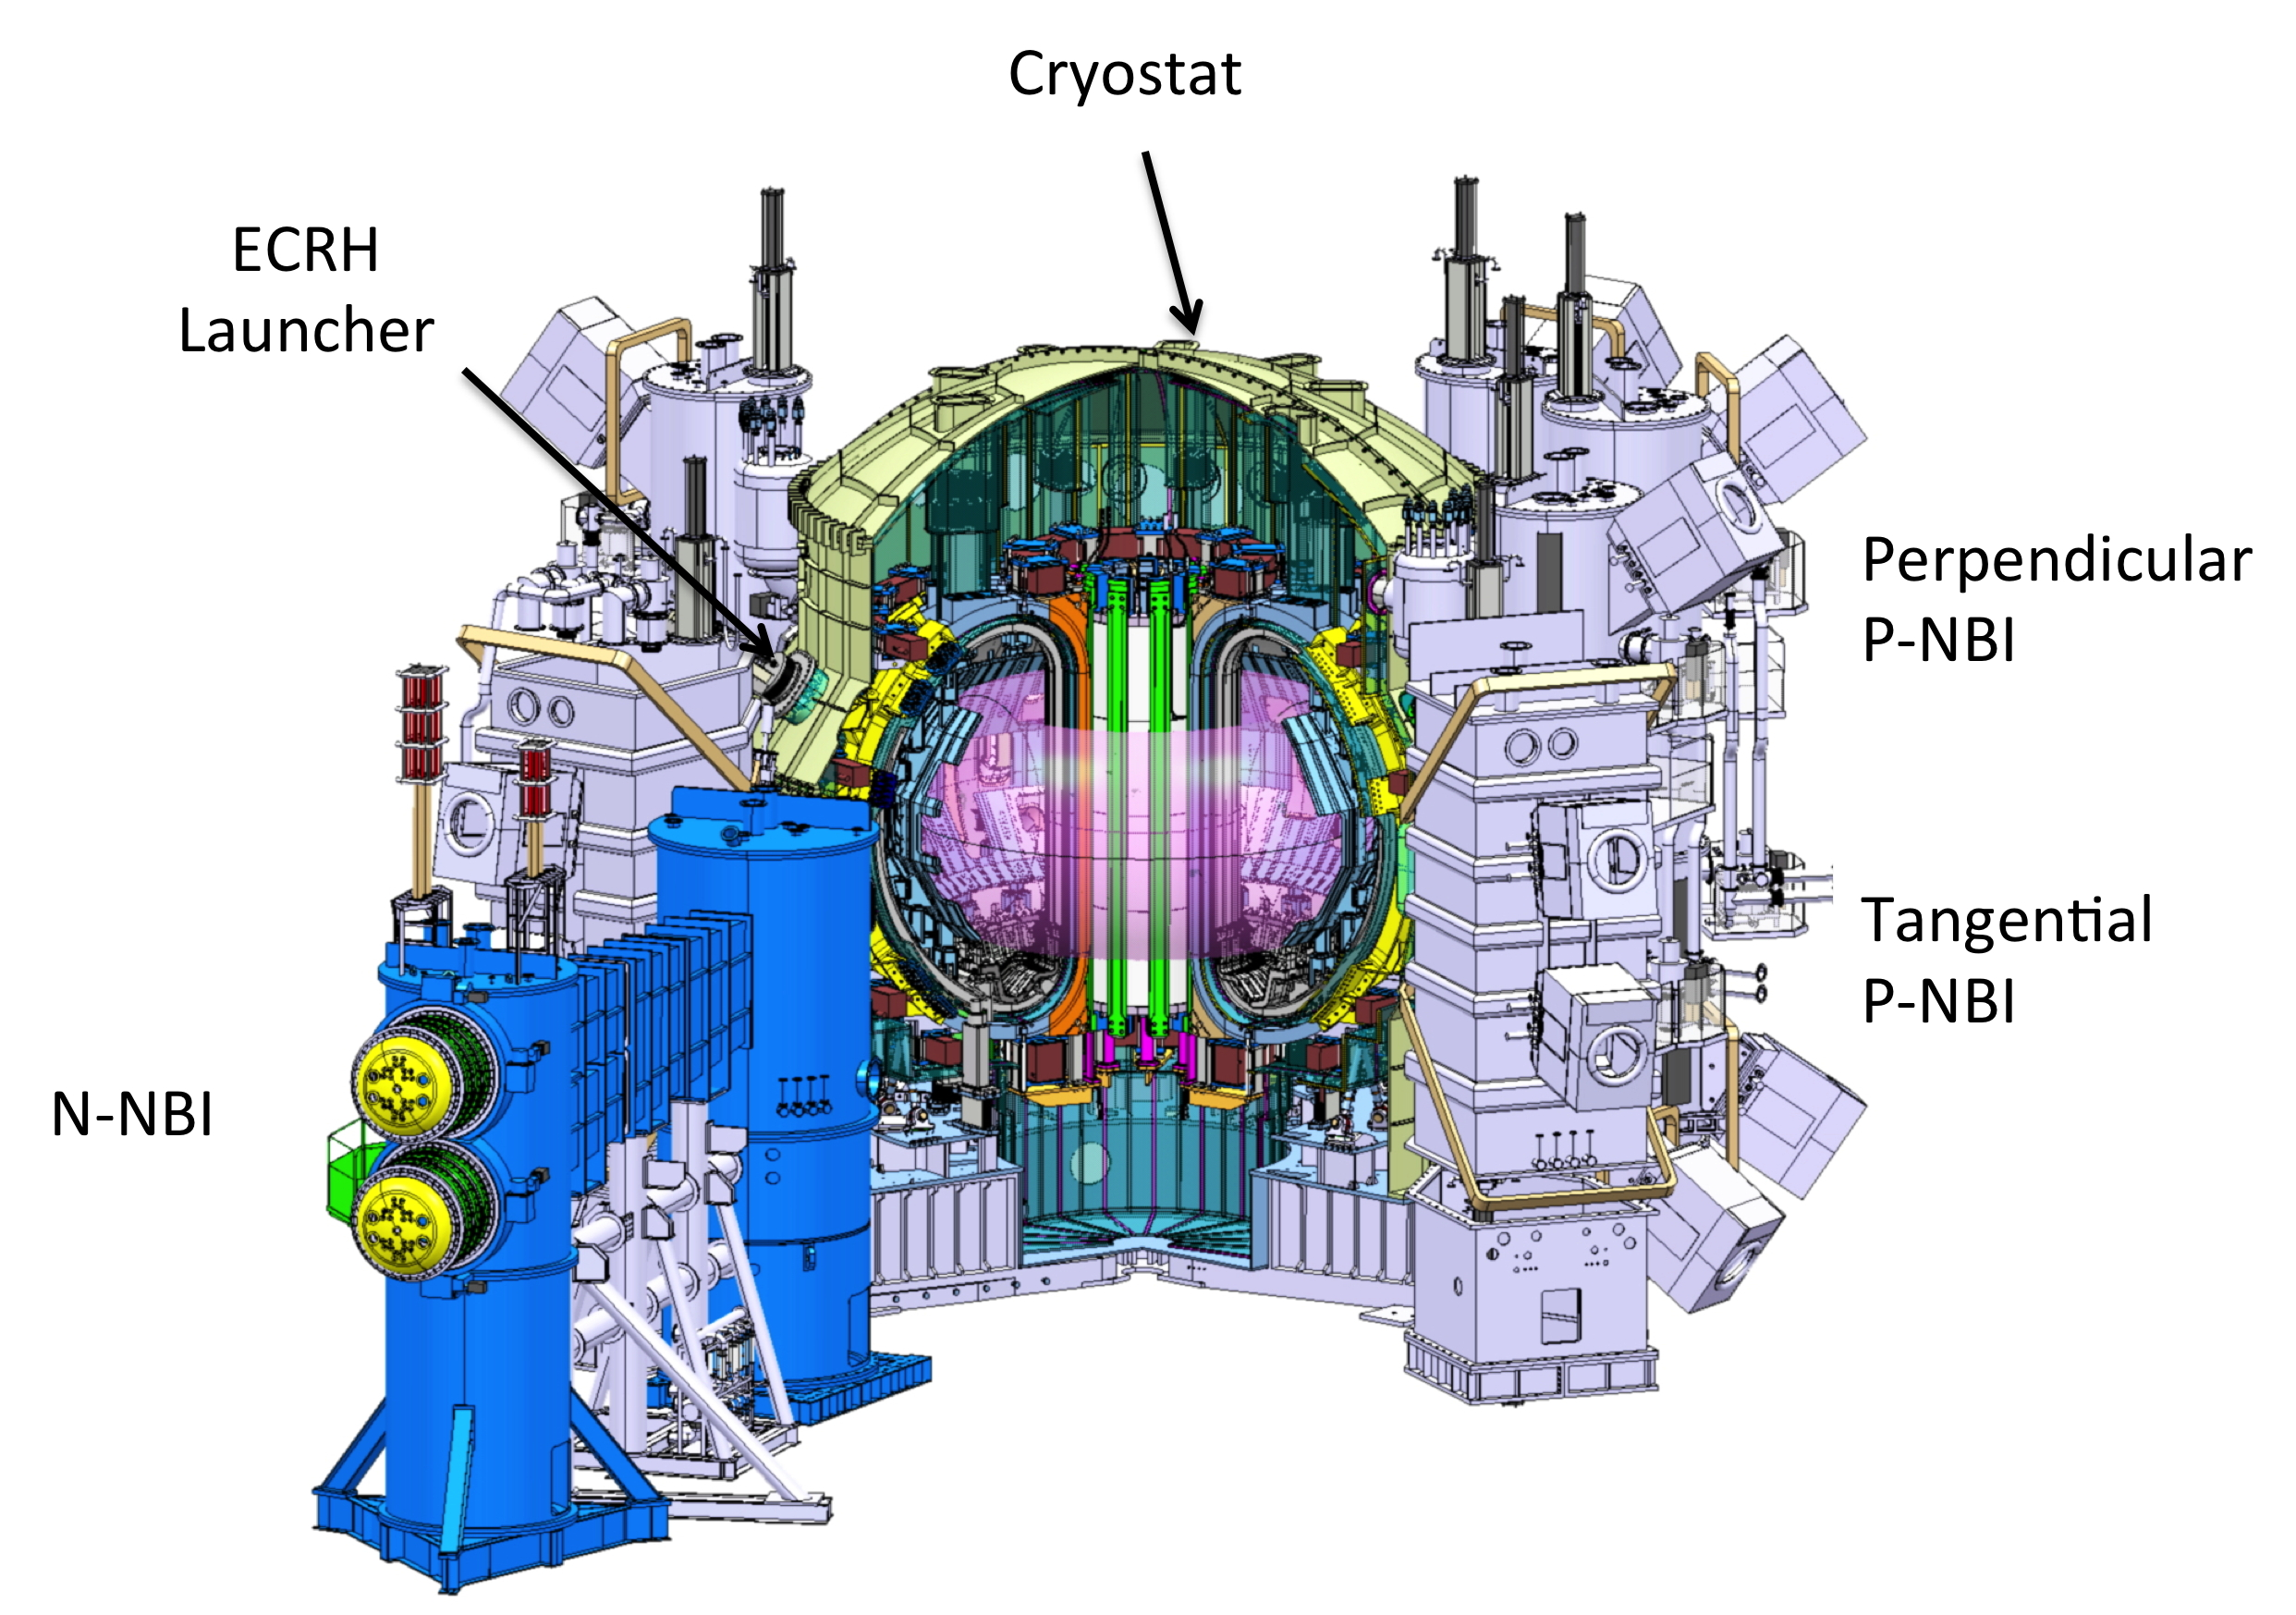
\includegraphics[width=0.75\textwidth]{Chp3/JT60SA.png}
	
	\caption{\label{JT60schm}JT60-SA tokamak configuration and its main elements ~\cite{JT60SA:ResearchPlan}.}
\end{figure}

The Poloidal Field (PF) coils shown in JT60-SA cross-section from figure ~\ref{JT60coils} consist of two sets of superconductive coils: the Equilibrium Field Coils (EF1–6) and the Central Solenoid (consisting of four independent coils, named CS1–4). Furthermore, two in-vessel Fast Plasma Position copper Coils (FPPC1–2) will also be installed ~\cite{NCruz}.The total of 12 PF coils have independent power sources value for the control of the plasma current, position and shape.   
\smallskip

\begin{figure}
	\centering
	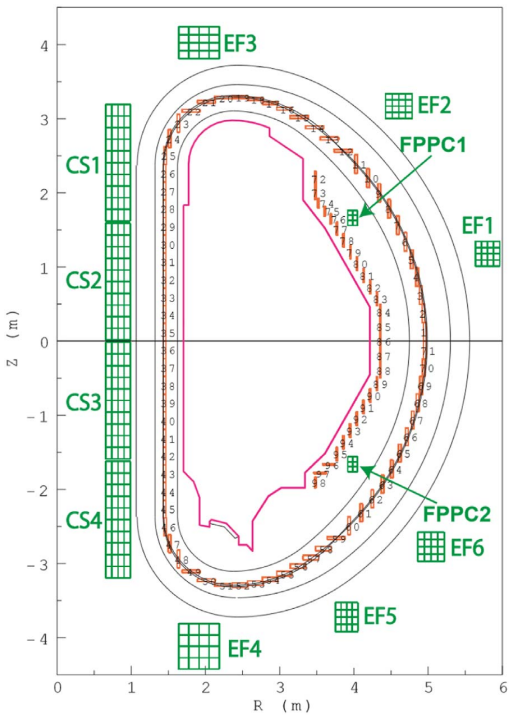
\includegraphics[width=0.55\textwidth]{Chp3/JT60Coils.png}

	\caption{	\label{JT60coils}JT-60SA poloidal cross-section and layout of the Poloidal Field coils system ~\cite{NCruz}.}
\end{figure}

JT-60SA shall be capable of investigating different design scenarios. As refereed  in 
~\cite{JT60SA:PID} it exists a set of 6 reference scenarios, additional ones, including some with a shorter repetition rate will be defined in future. For the control study in this section all simulations will be built based on the Scenario~2 characteristics. In particular, Scenario~2 refers to a~5.5 MA inductive lower single null discharge.The Scenario~2 its divided in 5 time snapshots with different equilibrium each one starting at  t=-40~s until t= 177.96~s. The different Last Closed Flux Surfaces (LCFS) for each time window are shown in figure~\ref{Scen2}, the time sequence starts at the X-point formation (XPF)	 followed by the Start of Heating(SOH), the Start of Flattop (SOF), End of Flattop (EOF), End Of Cooling(EOC) and finishing with the End of Currents in the PF coils (EOC). In this section reconstruction methods and control algorithms will be based on the \emph{Start of Flattop}~(SOF) equilibrium shown in figure~\ref{SOF}. The nominal values for the plasma current, the poloidal beta and the internal inductance for Scenario~2 at SOF are~$I_{p_{eq}}~=~5.5$~MA, $\beta_{p_{eq}}=0.53$, and~$l_{i_{eq}}=0.85$.\smallskip

\begin{figure}[h]
	\centering
	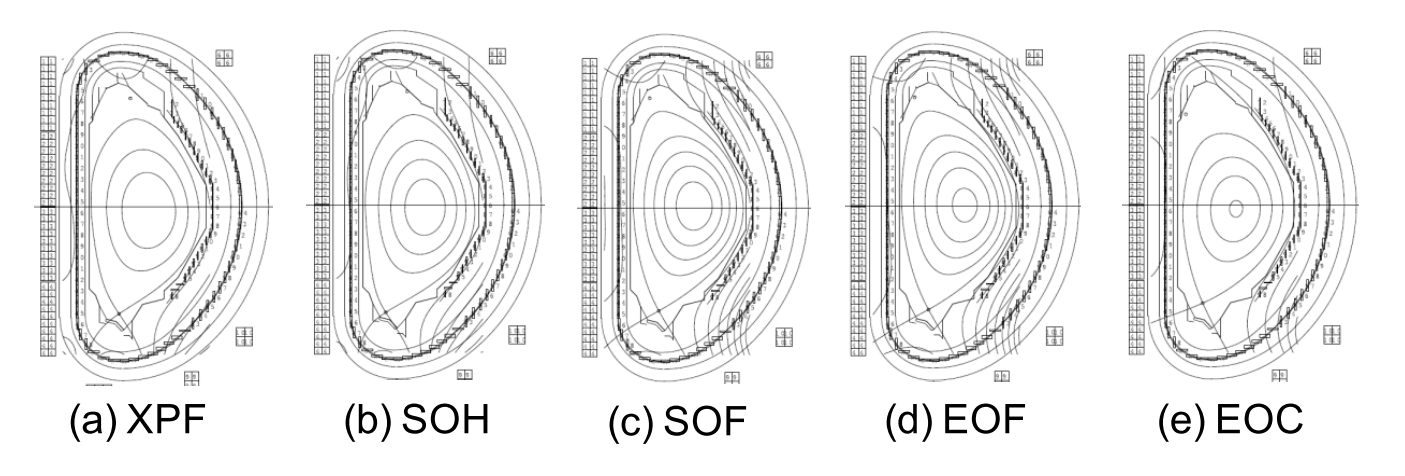
\includegraphics[width=0.99\textwidth]{Chp3/scenario2SnapShots.png}
	
	\caption{LCFS Equilibria corresponding to the different Scenario~2 snapshots:  X-point formation (XPF), Start of Heating(SOH), the Start of Flattop (SOF), End of Flattop (EOF), End Of Cooling(EOC) and  End of Currents in the PF coils (EOC). \label{Scen2}}
\end{figure}


\begin{figure}[h]
	\centering
	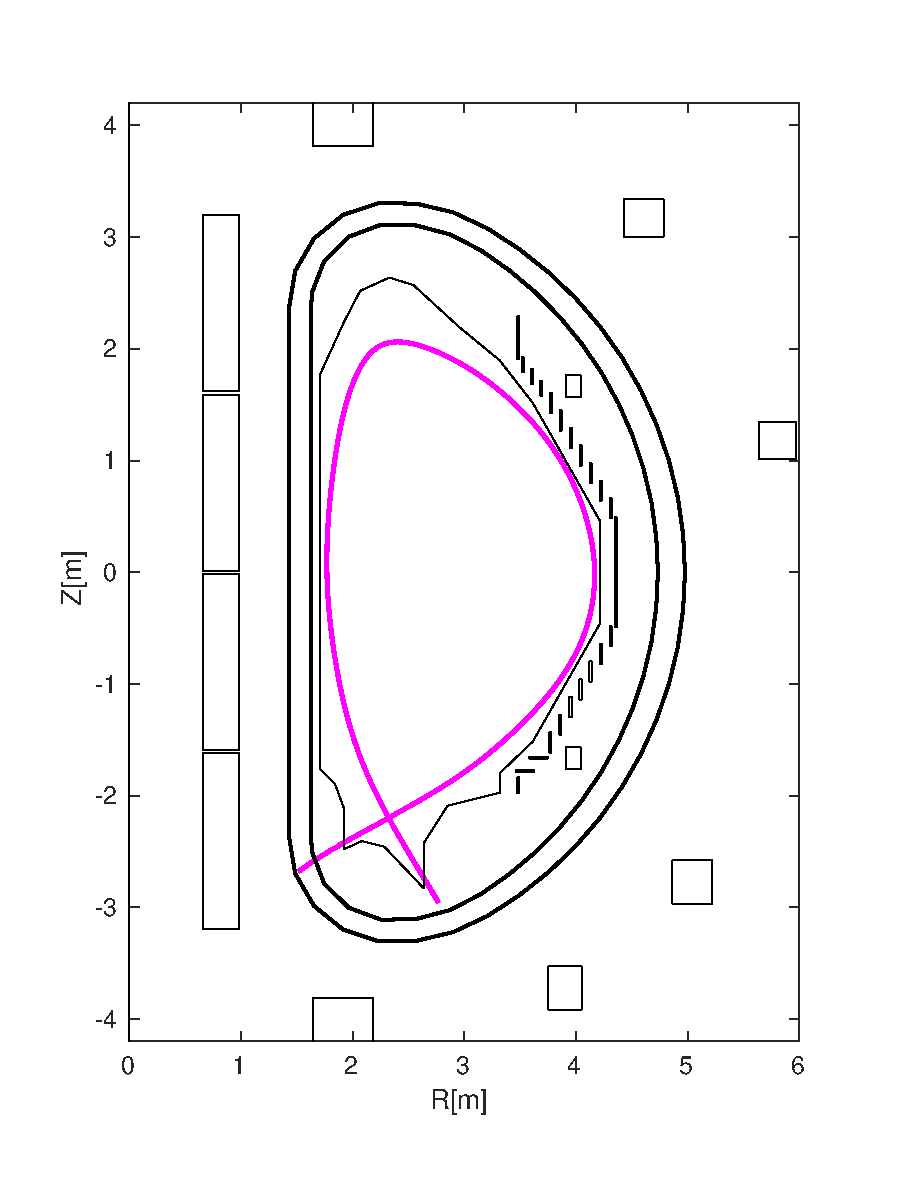
\includegraphics[width=0.5\textwidth]{Chp3/scenario2_SOF.eps}
	
	\caption{Poloidal cross-section of the JT-60SA plasma at the Start of the Flat Top~(SOF) for reference Scenario~2. At SOF, the nominal plasma current is~5.5~MA, while the nominal values for poloidal beta~$\beta_p$ and internal inductance~$l_i$ are~0.53 and~0.85, respectively.	\label{SOF}}
\end{figure}



This chapter will address two different approaches for the LCFS reconstruction along  with different plasma current, shape and position controllers on  JT60-SA in order to achieve and maintain the desired operational scenario given the plasma equilibrium in the SOF while the performance of the controllers is compared .



\section{CREATE magnetic reconstruction tools}

CREATE-NL (Consorzio di Ricerca per l' Energia, l' Automazione e le Tecnologie dell' Elettromagnetismo) is a finite elements method (FEM\footnote{It is well known that many physical and engineering systems are expressed in terms of partial differential equations which cannot be solved via analytical methods. One of the most recurrent techniques is numerical discretization to approximate the solution of the partial differential equations, the FEM is commonly used to solve these approximations in two or three space variables, in this particular case for a numerical solution of the well-known Grad-Shafranov equation. }) solver implemented on \textsc{Matlab}. It deals with the free boundary dynamic plasma equilibrium problem i.e. the MHD (Magneto Hydro Dynamics) time evolution of 2D axisymmetric plasmas in tokamaks, including eddy currents in the passive structures, and feedback control laws for current, position and shape control ~\cite{Albanese:CREATENLnew}.
\smallskip

Using the CREATE codes~\cite{Albanese:CREATEL,Albanese:CREATENLnew} it is possible to retrieve a linearized state-space model that describes the plasma magnetic behavior around that equilibrium\footnote{Reference  ~\cite[Sec.~3]{NCruz} can be consulted for more details about the use of the CREATE equilibrium codes to retrieve plasma linearized models.}.It shoudl be noted that CREATE-NL equilibrium solver has been validated on several tokamaks such as JET and EAST.
\smallskip

A JT60-SA CREATE-NL electromagnetic linear model around the equilibrium from the Scenario~2-~SOF  for the plasma-circuit response has been used for  designing  the controller presented in next section.




\section{Controller design}

The JET (Joint European Torus) tokamak was the first machine where around 2005 a new model based plasma current and shape controller was set up and tested  with the existing active circuits and control hardware. The novelty controller was the eXtreme Shape Controller (XSC) and its aim was to improve  the performance of the back then present controller to allow the control of extremely shaped plasmas with higher values of elongation and triangularity ~\cite{Albanese2005}. More recently this control approach was utilized at TCV ~\cite{anand2017novel}. At JET, the XSC recently enabled the control of high triangularity shapes with both strike points in the divertor corner, which has a large impact in the H-mode confinement in the case of ITER-like wall at JET~\cite{de2016recent}.   
 \smallskip
 
 Usually the controlled shape geometrical descriptors are the distances between the plasma boundary and the vessel at some specific points. These plasma-wall distances are called gaps ~\cite{Ambrosino:TCST2008}. The gaps are segments that can be used to describe the shape of the plasma boundary. Being~$g_i$ the abscissa along the~$i$-th control segment, we assume that~$g_i=0$ at the first wall. \emph{Gap-based} plasma shape control is achieved by controlling to zero the difference $g_{i_{ref}}-g_i$ on a sufficiently large number of gaps, being~$g_{i_ref}$ the value of the abscissa on the~$i$-th control segment for the reference shape. Figure ~\ref{figure:85_gaps} shows a poloidal cross-section of JT-60SA together with a set of 85 gaps used for the assessment of the plasma shape control.
 \smallskip
 
 \begin{figure}[h]
 	\begin{center}
 		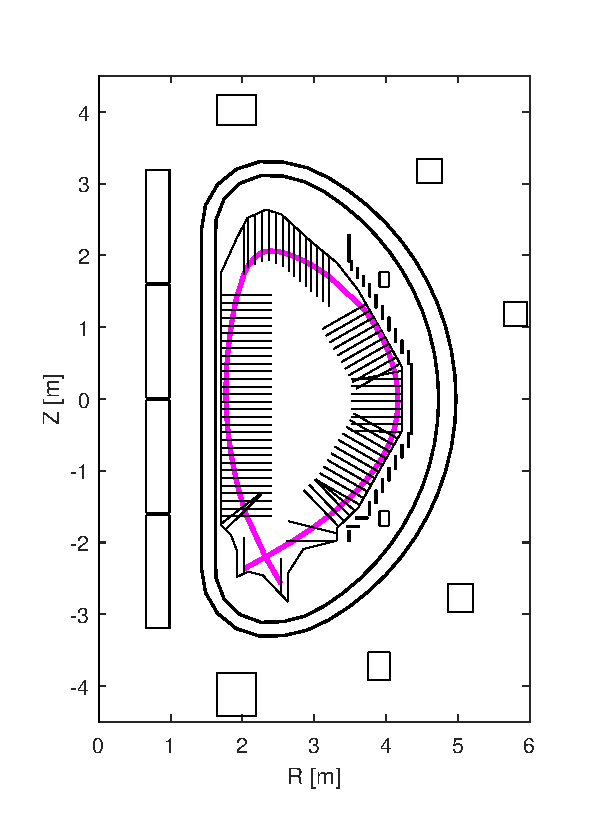
\includegraphics[width=0.45\textwidth]{Chp3/85_gaps_2.eps}
 	\end{center}\caption{Poloidal cross-section of the JT-60SA plasma at the Start of the Flat Top~(SOF) for reference Scenario~2. At SOF, the nominal plasma current is~5.5~MA, while the nominal values for poloidal beta~$\beta_p$ and internal inductance~$l_i$ are~0.53 and~0.85, respectively. In this figure the~85 gaps used to assess the plasma shape controller performance are shown.}\label{figure:85_gaps}
 \end{figure}
 
  The XSC algorithm can be used either to implement a gap-based control strategy, or an isoflux one, as it has been proposed in ~\cite{NCruz}. The isoflux strategy consists in controlling the X-point position along with a set of flux differences between the flux at some selected control points along the desired plasma boundary and the X-point flux.
\smallskip


The peculiarity of the XSC approach is that it permits to control a number of plasma shape descriptors that is greater than the number of available actuators, i.e. of PF Circuits, this  is basically tackled by using a singular value decomposition (SVD) to identify the principal directions of the algebraic mapping between coil currents and geometrical descriptors ~\cite{Albanese2005}. The XSC control relies on the PFC decoupling controller (more details can be found in~\cite[Section~4.4]{NCruz}), since it is assumed that each~PFC can be treated as an independent single-input-single-output channel whose dynamic response is modeled in the Laplace domain by
\[
I_{PF_i}(s) = \frac{I_{PF_{ref\,,i}}(s)}{1+s\tau_{PF}}\,,
\]
where~$I_{PF_i}$ and~$I_{PF_{ref_i}}$ are the Laplace transform of the measured and reference current in the~$i$-th PFC, respectively, and where it is assumed that all the PFC exhibit the same bandwidth (i.e.,~they have the same time constant~$\tau_{PF}$).
\smallskip

Denoting by~$\delta Y(s)$ the Laplace transform of the variations of the~$n_G$ gaps to be controlled, it is possible to exploit the CREATE electromagnetic linear model~\cite{NCruz} that links the variation of the PFC reference currents~$\delta I_{PF_{ref}}$ to ~$\delta Y(s)$, i.e.
\[
\delta Y(s) = C\frac{\delta I_{PF_{ref}}(s)}{1+s\tau_{PF}}\,,
\]
which, at steady-state, implies~ $\delta Y(s) = C \delta I_{PF_{ref}}(s)$.

If the number of controlled plasma shape descriptors~$n_G$ is such that~$n_G~>~n_{PF}$, the XSC computes the additional current references as
\begin{equation}\label{equation:XSC_new}
\delta I_{PF_{ref}}=C^\dag\delta Y\,.
\end{equation}
where the matrix~$C^\dag$ denotes the pseudo-inverse of~$C$\footnote{$C$ is the output matrix from the state-space linearized CREATE model for JT60-SA.} that can be computed via the singular value decomposition (SVD). As a result, the XSC algorithm minimizes the following
steady-state performance index
\begin{equation}\label{equation:XSCcost}
J_{XSC} = \lim_{t\to +
	\infty}(\delta Y_{ref}-\delta Y(t))^T(\delta Y_{ref}-\delta Y(t))\,,
\end{equation}
where~$\delta Y_{ref}$ are constant references for the geometrical descriptors. When the SVD of the~$C$ matrix is used to minimize~\eqref{equation:XSCcost}, it may happen that some singular values (depending on the plasma configuration) are one order of magnitude smaller than the others. This fact implies that minimizing the performance index~\eqref{equation:XSCcost} retaining all the singular values results in a large control effort at the steady-state, that is a large request on some PFC currents which have only a minor effect on the plasma shape. In order to minimize also the control effort, the additional references~\eqref{equation:XSC_new} are generated by using only the~$\bar{n}<n_{PF}$ linear combinations of PF currents which are related to the largest singular values of the~$C$ matrix. This is achieved by using only the~$\bar{n}$ singular values when computing the pseudo-inverse~$C^\dag$.
\smallskip

Moreover, the PFC current variations given by~\eqref{equation:XSC_new} are summed to the scenario currents and sent to the PFC decoupling controller as references to be tracked. It is worth to remark here that the dynamnic behaviour of the XSC is improved by adding a set of proportional-integral-derivative (PID) controllers on each PFC channel (see~\cite{Ariola:XSC} for a complete description of the XSC control scheme).
\smallskip

For the development of this work both approaches of the XSC strategy were studied and simulated for a different number of control points: isoflux and gap-based controllers. In addition, a second controller developed by the QST team was implemented in the simulations, the features of this controller will be detailed in the next section.



\section{QST reconstruction and control implementation}

Along with the CREATE tools presented above  for the reconstruction of the LCFS and the XSC for plasma shape control, a reconstruction code and controller provided by the QST team were tested and compared. This section will briefly describe these two methods and its limitations.  

\subsection{Cauchy Condition Surface reconstruction  method }
The QST Cauchy Condition Surface (CCS) method for the reconstruction of the magnetic last closed flux surface calculates controlled variables for plasma position and shape control such as the poloidal magnetic flux at control points on an isoflux scheme  ~\cite{CCS} . The CCS method allows a selection up to 19 geometrical control points and its input parameters are the current in the PF coils, the measurements in the magnetic field and flux sensors and the plasma current. The output signals from the CCS reconstruction method are the magnetic fluxes at the X-point an the selected control points. 

\begin{figure}
	\centering
	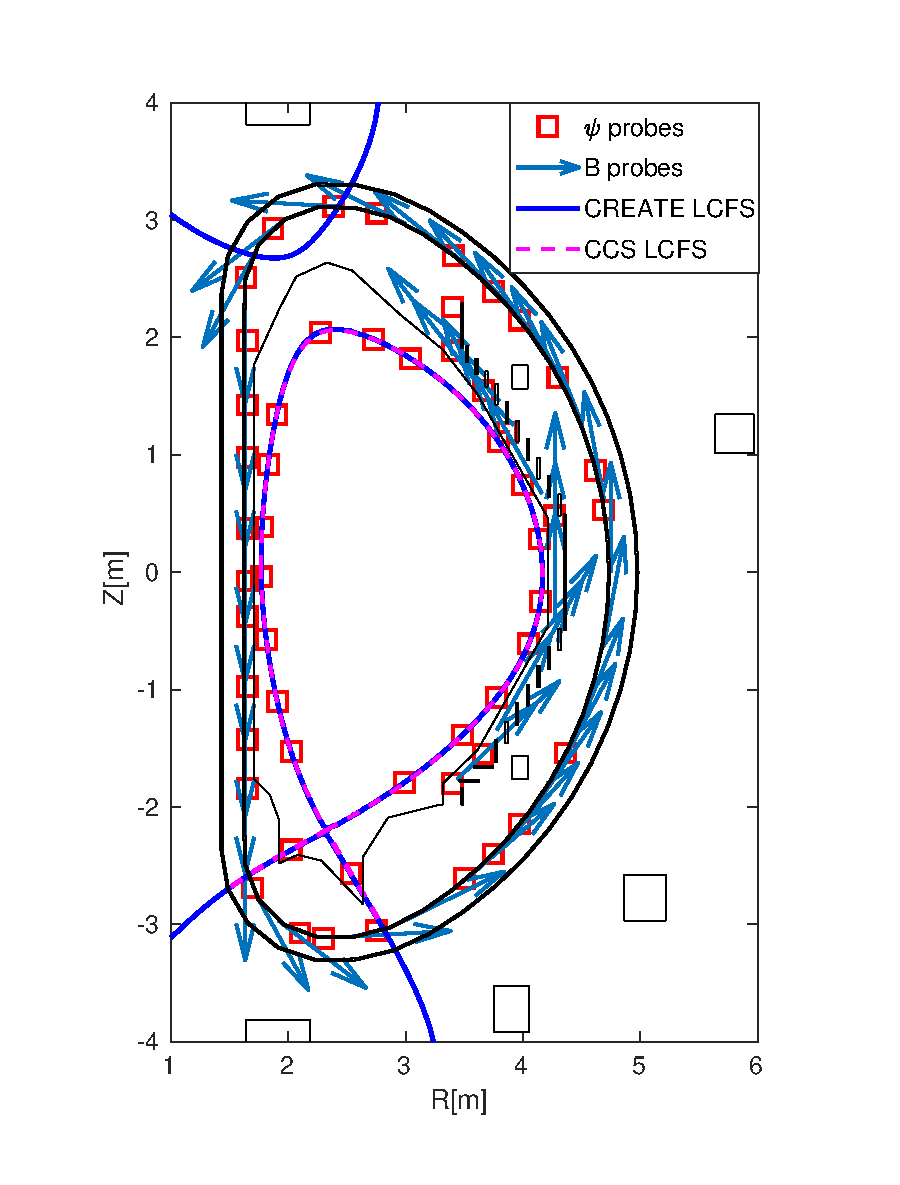
\includegraphics[width=0.7\textwidth]{Chp3/sensors_plots_newDirection.eps}
	\caption{SOF equilibrium reconstructed from CREATE-NL and the CCS code along with the  magnetic field and flux sensors locations	\label{JT60sensors} }
\end{figure}


\subsection{QST magnetic controller (FBC)}


The QST magnetic controller FBC uses the PF coils signals to control the plasma current $I_p$ and the FPPC coils signals for plasma position control ~\cite{FBC}.

QST magnetic controller calculates command values of active coil ccurrents/voltages from some information

\begin{equation}
I_{PF\_ref}(t+\Delta t) = I_{PF}(t_0)+M^\dagger_{PF}\left[G_{SP}\delta\Psi_s(t)+G_{SI}\int_{t_0}^{t}\delta\Psi_s(t)dt+G_{XP}\delta\Psi_X(t)+G_{XI}\int_{t0}^{t}\delta\Psi_x(t)dt\right]
\end{equation}

\begin{equation}
V_{com}=G_{vt}\left[M_{coil}\frac{(I_{coil\_ref}-I_{coil\_meas})}{dt}+ \frac{M_{plasma\_now} \cdot I_{p\_now} - M_{plasma\_ bfr} \cdot I_{p\_bfr}}{dt}\right]
\end{equation}

\begin{equation}
I_{FPPC\_ref}(t+\Delta t)=I_{FPPC}(t_0)+ M^\dagger_{FPPC}\left[G_{FP}\delta \Psi_{SF}(t) + G_{FD}\frac{d}{dt}\delta\Psi_{SF}(t) \right]
\end{equation}





\section{Simulation results}	

 The simulations for  the JT60-SA CREATE-NL model ,the XSC, the CCS reconstruction method and the QST controller  were programmed on top of  \textsc{Matlab} and \textsc{Simulink} blocks. This  section will address in detail the outcome of the control simulations 
 
 
\begin{figure}
	\centering
	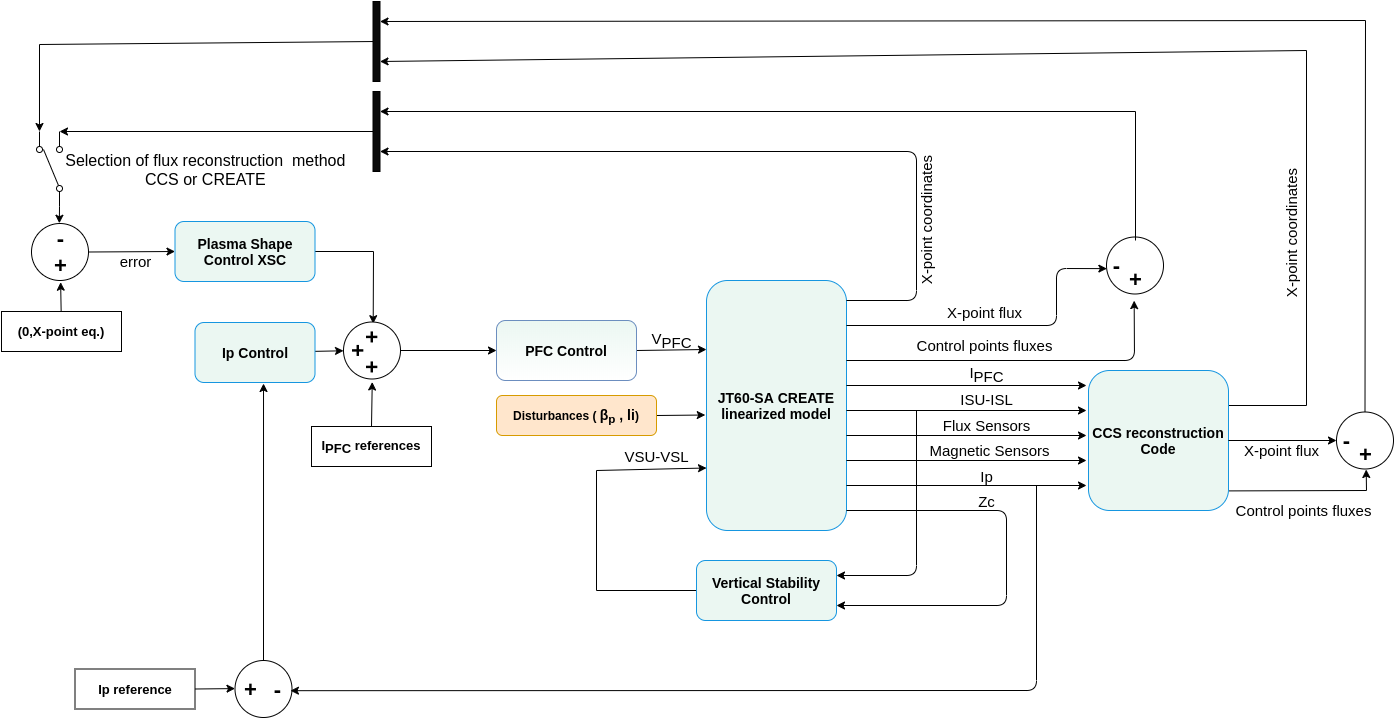
\includegraphics[width=1.05\textwidth]{Chp3/JT60Schemes1.png}
	\caption{	\label{JT60controlscheme}JT-60SA }
\end{figure}

\begin{figure}
	\centering
	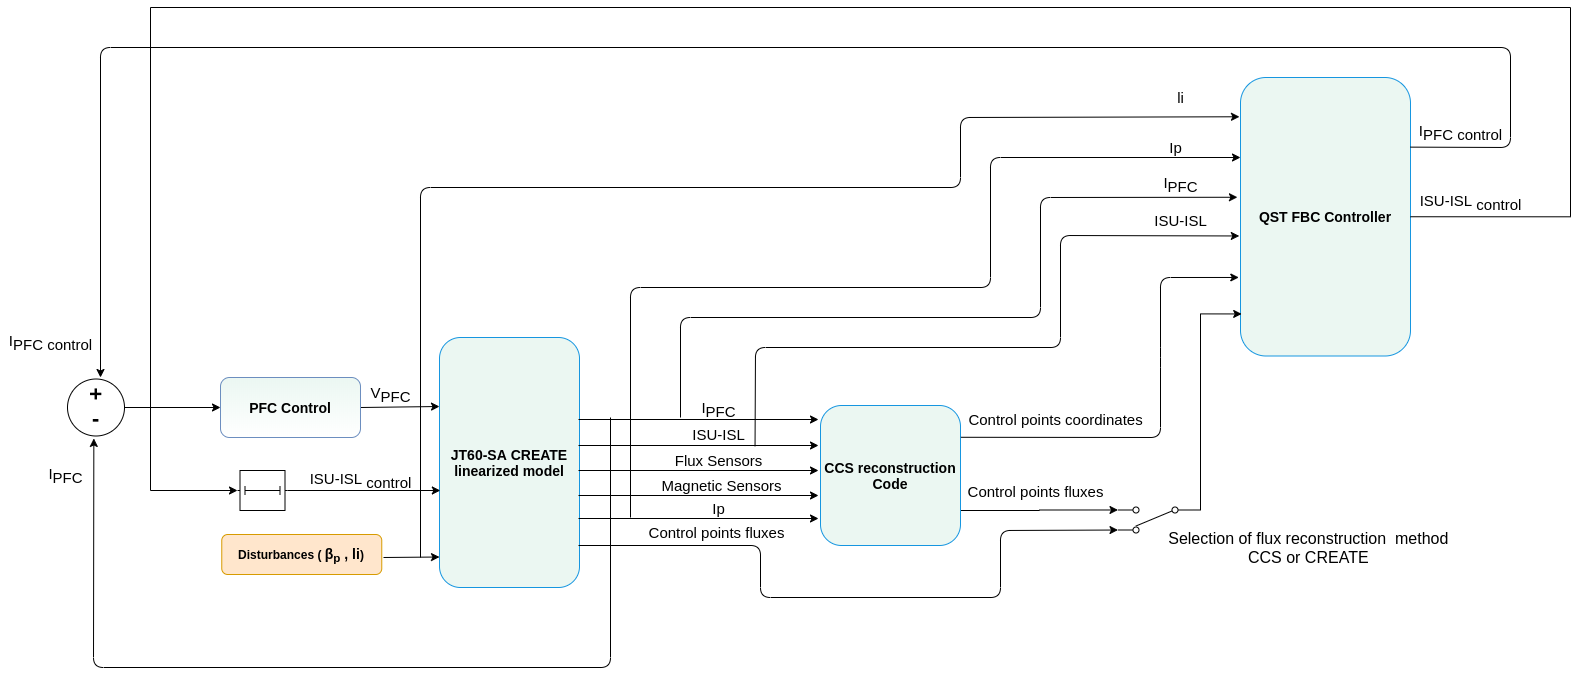
\includegraphics[width=1.05\textwidth]{Chp3/JT60SchemeFBCnew.png}
	\caption{	\label{JT60FBCcheme}JT-60SA }
\end{figure}



\subsection{Disturbances}

\begin{itemize}
	\item \textbf{Disturbance \#1} refers to the behaviour of~$\beta_p$ and~$l_i$ soon after the current flattop is reached, as it was modeled in~\cite{urano2015development} (in this paper we assume that the flattop is reached at~$t\sim 16$~s). As an example, the correspondent time traces are shown in Fig.~\ref{figure:Urano}\footnote{The time behaviour of both~$\beta_p$ and~$l_i$ have been estimated starting from the spatial profiles for both plasma density and temperature envisaged for Scenario 2.}.
	
	\item \textbf{Disturbance \#2} refers to the behaviour of ~$\beta_p$  due to the presence of an Edge-Localized Mode~(ELM). As described in~\cite[p.~34]{JT60SA:PID}, during the flattop an instantaneous drop in~$\beta_p$ of ~$0.05~\beta_{p_{eq}}$ is followed by and exponential recovery with a time constant of~0.05~s with a frequency 10~Hz. Note that for this disturbance~$l_i$ does not change.% remains as~$l_{i_{eq}}$, these behaviors are shown in Fig.~\ref{figure:ELM}.
	
	\item \textbf{Disturbance \#3} refers to the behaviour of~$\beta_p$ and~$l_i$ when a compound ELM\footnote{A compound ELM is commonly referred as multiple clearly distinguishable
	crash events causing large energy losses \cite{Meyer2017}.} appear during the flattop~\cite[p.~34]{JT60SA:PID}. The time trace of~$\beta_p$ is the same as in the case of Disturbance~\#2, $l_i$ is described by an instantaneous drop of~$0.06~(l_{i_{eq}}-0.5)$ followed by and exponential recovery with a time constant of 0.05~s with a frequency 10~Hz. 
	The time traces for~$\beta_p$ and~$l_i$ are described in Fig.~\ref{com_ELM}.
	
%	\item \textbf{Disturbance \#3} describes an instantaneous drop in~$l_i$ of~$0.2~(l_{i_{eq}}-0.5)$ without recovery, simultaneous with a drop on~$\beta_p$ of~$0.2~\beta_{p_{eq}}$ followed by a recovery exponential time of~1~s~\cite[p.~34]{JT60SA:PID}, which are typical of a so called \emph{minor disruption}. %The correspondent time traces for both~$\beta_p$ and~$l_i$ are reported in Fig.~\ref{figure:minor_dis}.
\end{itemize}

\begin{figure}
	\centering
	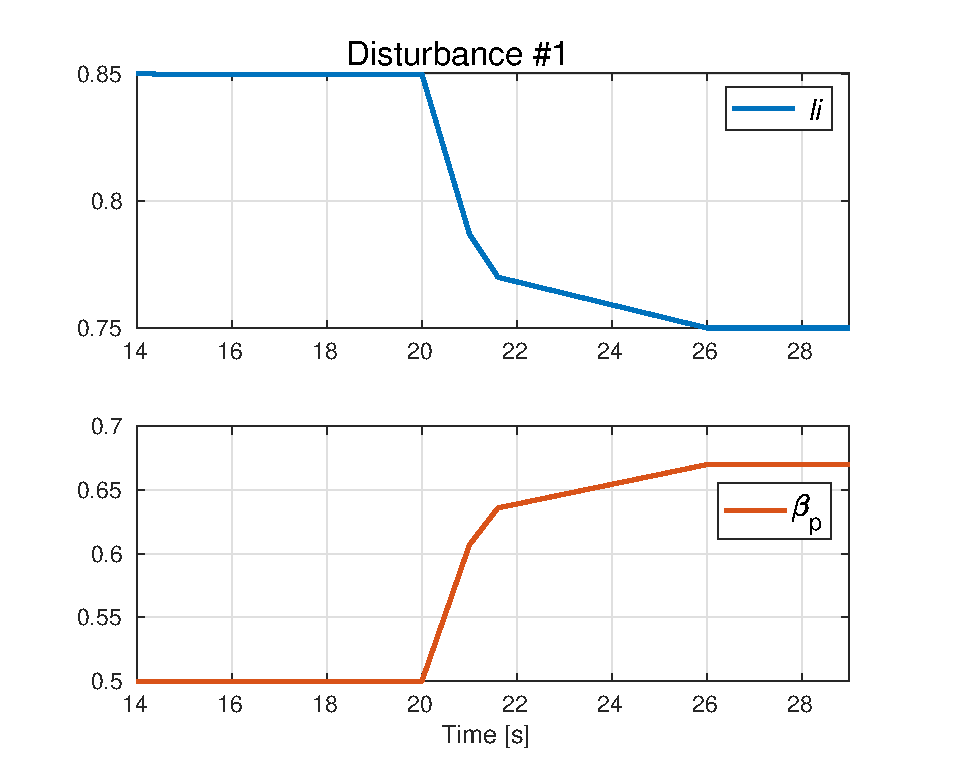
\includegraphics[width=0.5\textwidth]{Chp3/Dist_1_Urano.eps}
	\caption{	\label{Urano} }
\end{figure}

\begin{figure}
	\centering
	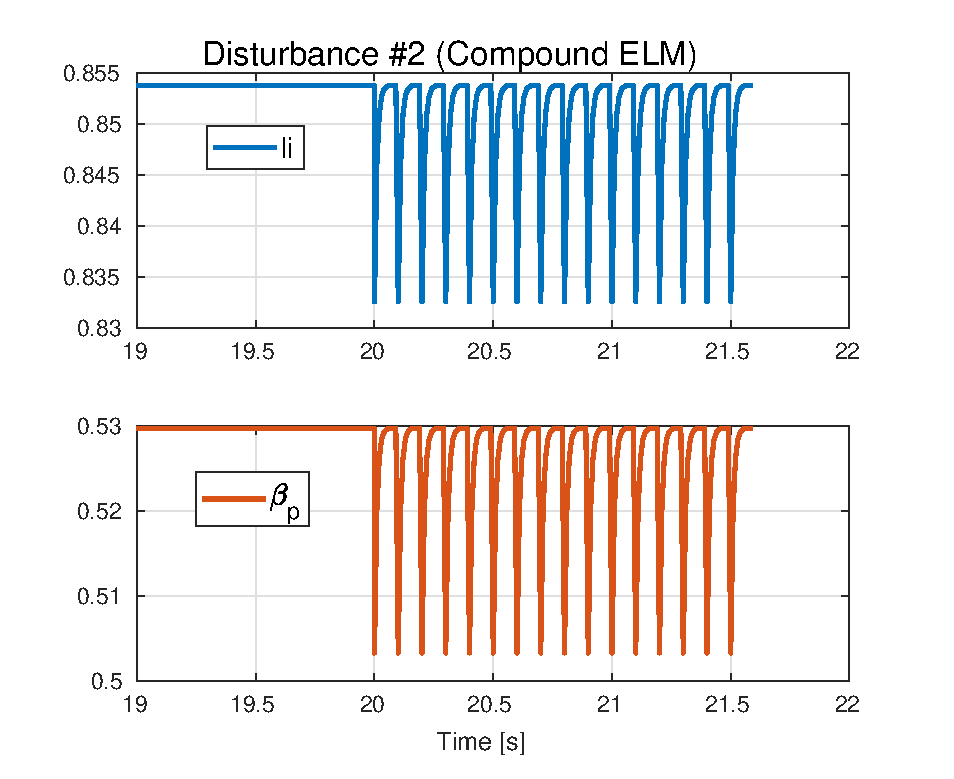
\includegraphics[width=0.5\textwidth]{Chp3/Dist_2_cmp_ELM.eps}
	\caption{	\label{cmpELM} }
\end{figure}


\begin{figure}
	\centering
	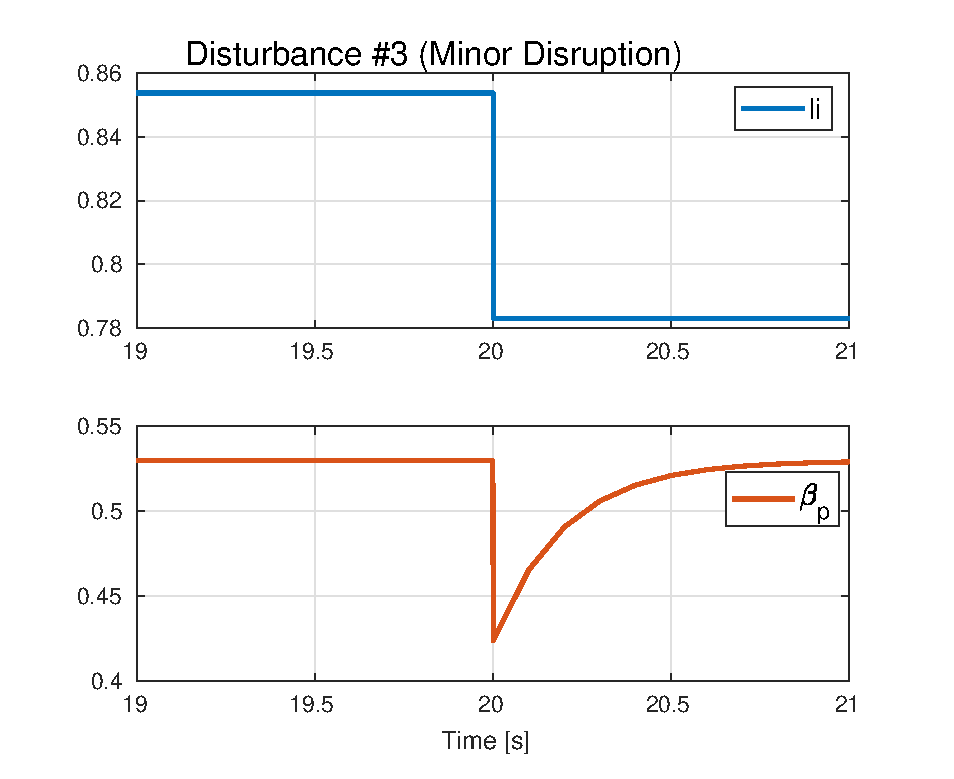
\includegraphics[width=0.5\textwidth]{Chp3/Dist_3_minor.eps}
	\caption{	\label{MnrDisrp} }
\end{figure}



\subsection{Gap-based XSC}



\begin{figure}
	\centering
	\begin{subfigure}[b]{0.32\textwidth}
		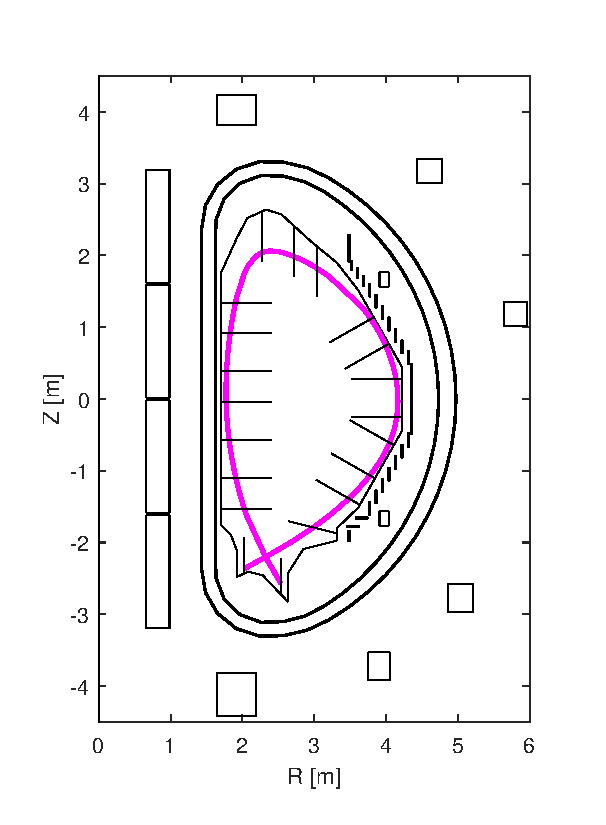
\includegraphics[width=\textwidth] {Chp3/20_gaps.eps}  
		\caption{The~20 gaps used to assess the performance of plasma shape controller.	\label{figure:20_gaps} }
	\end{subfigure}
	~
	\begin{subfigure}[b]{0.32\textwidth}
		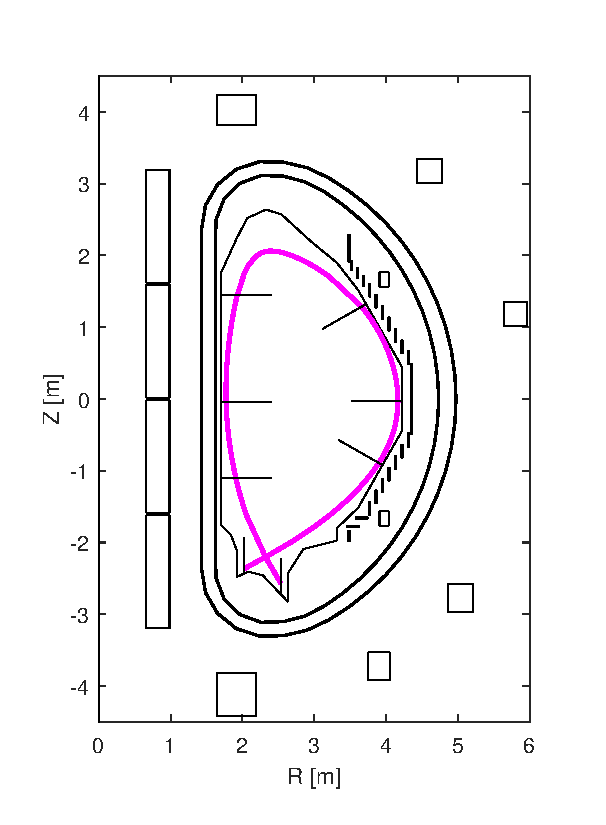
\includegraphics[width=\textwidth]{Chp3/8_gaps.eps} 
		\caption{The~8 control segments by the isoflux controller proposed in~\cite{miyata2013study}.\label{figure:8_gaps}}
	\end{subfigure}
	~
	\begin{subfigure}[b]{0.32\textwidth}
		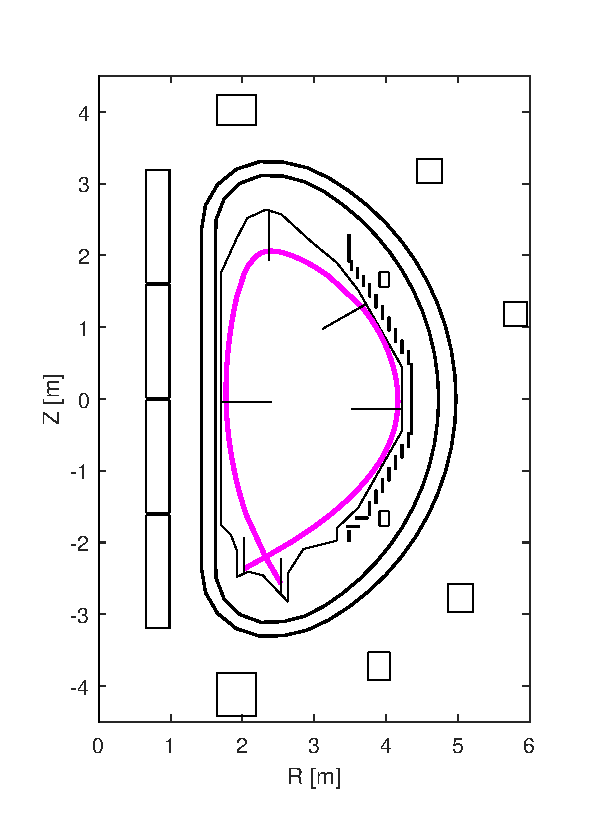
\includegraphics[width=\textwidth]{Chp3/6_gaps.eps} 
		\caption{ The~6 control segments used by the isoflux controller proposed in~\cite{Miyata:2014}. \label{figure:6_gaps}}
	\end{subfigure}
	
\caption{Different choices for the set of controlled gaps used for gap controller.} \label{figure:gapChoices}
\end{figure}




\begin{figure}
	\centering
	\begin{subfigure}[b]{0.32\textwidth}
		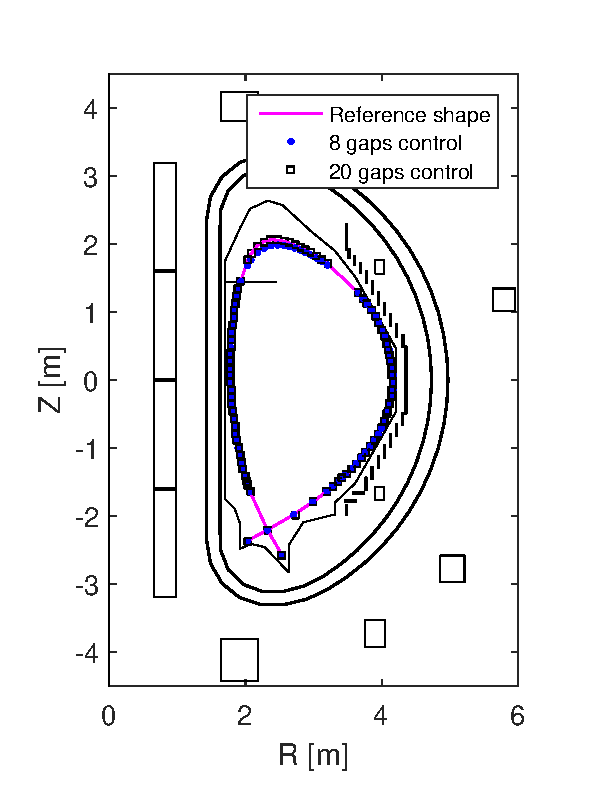
\includegraphics[width=\textwidth] {Chp3/Ref_20gaps_8gaps_minor_2.eps}  
		\caption{Poloidal cross-section of JT-60SA.\label{figure:minor_big} }
	\end{subfigure}
	~
	%	~ %add desired spacing between images, e. g. ~, \quad, \qquad, \hfill etc. 
	%(or a blank line to force the subfigure onto a new line)
	\begin{subfigure}[b]{0.32\textwidth}
		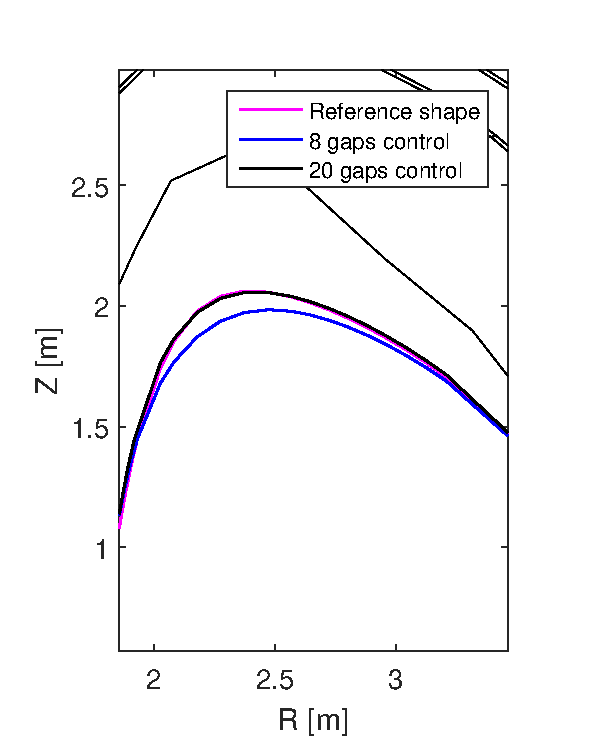
\includegraphics[width=\textwidth]{Chp3/zoom_Ref_20gaps_8gaps_minor_top_2.eps} 
		\caption{Detailed view of the plasma top region.\label{figure:minor_big}}
	\end{subfigure}
	~
	\begin{subfigure}[b]{0.32\textwidth}
		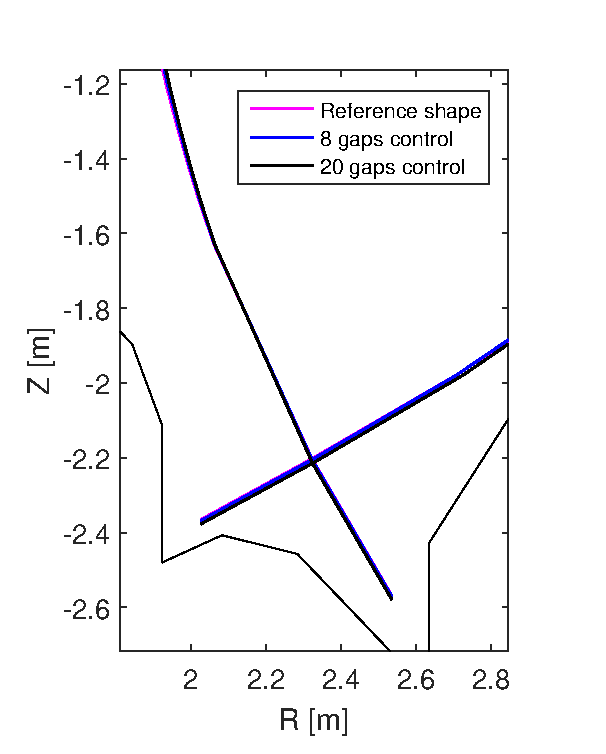
\includegraphics[width=\textwidth]{Chp3/zoom_Ref_20gaps_8gaps_minor_strike_2.eps} 
		\caption{Detailed view of the plasma divertor region. \label{figure:minor_strike}}
	\end{subfigure}
	
	
	\caption{ Comparison of the shape controller performance in the presence of Disturbance~\#3 (minor disruption). The two cases of 8 and 20 gaps are considered.}
\end{figure}

\subsection{Isoflux XSC and QST controller }



% Please add the following required packages to your document preamble:
% \usepackage[table,xcdraw]{xcolor}
% If you use beamer only pass "xcolor=table" option, i.e. \documentclass[xcolor=table]{beamer}
\begin{table}[]
	\centering
	\begin{tabular}{|l|c|c|c|c|c|c|c|c|}
		\hline
			\rowcolor{color2}
		\multicolumn{9}{|c|}{\textbf{Disturbance $\#3$ (Minor disruption) steady state X-point error}}                                                                                                                                                                         \\ \hline
			\rowcolor{color1}
		Controller                                                            & \multicolumn{4}{c|}{eXtreme Shape Controller}          & \multicolumn{4}{c|}{QST Controller}                                                                       \\ \hline
			\rowcolor{color3}
		\begin{tabular}[c]{@{}l@{}}LCFS reconstruction \\ method\end{tabular} & \multicolumn{2}{c|}{CCS} & \multicolumn{2}{c|}{CREATE} & \multicolumn{2}{c|}{CCS}                            & \multicolumn{2}{c|}{CREATE}                         \\ \hline
		& Rx mm       & Zx mm      & Rx mm        & Zx mm        & Rx mm                    & Zx mm                    & Rx mm                    & Zx mm                    \\ \hline
		6 points       &                                                       -4.92           & 20.9          & -3.57            & 28.8              & -2.70                        & -0.105                        & -2.24                        &   0.369                      \\ \hline
		8 points                                                              &17.44           & 21.56          & 17.81            & 29.04           &   47.08                      &     -46.56                     & 57.61                       &           -41.42              \\ \hline
		19 points                                                             &-5.54           & 16.78          & -4.42           & 24.41             & \cellcolor[HTML]{C0C0C0} & \cellcolor[HTML]{C0C0C0} & \cellcolor[HTML]{C0C0C0} & \cellcolor[HTML]{C0C0C0} \\ \hline
	\end{tabular}
\caption{X-point position steady state error for a given JT60-SA scenario in the presence of a minor disruption. The XSC and  QST controller were used in different simulations for the shape control along  with two reconstruction methods for the LCFS. }
\end{table}


%\begin{table}[]
%	\centering
%	\begin{tabular}{|l|c|c|c|c|c|c|}
%		\hline
%		\rowcolor{color2}
%		\multicolumn{7}{|c|}{\textbf{Minor disruption steady state error}}                                                                                                                   \\ \hline
%		\rowcolor{color1}
%		Controller                                                            & \multicolumn{4}{c|}{eXtreme Shape Controller}          & \multicolumn{2}{l|}{QST Controller}                 \\ \hline
%		\rowcolor{color3}
%		\begin{tabular}[c]{@{}l@{}}LCFS reconstruction \\ method\end{tabular} & \multicolumn{2}{c|}{CCS} & \multicolumn{2}{c|}{CREATE} & \multicolumn{2}{c|}{CCS}                            \\ \hline
%		& Rx mm       & Zx mm      & Rx mm        & Zx mm        & Rx mm                    & Zx mm                    \\ \hline
%		6 points                                                              & -4.92           & 20.9          & -3.57            & 28.8            & xxx                        & xxx                        \\ \hline
%		8 points                                                              & 17.44           & 21.56          & 17.81            & 29.04            & xxx                        & xxx                        \\ \hline
%		19 points                                                             & -5.54           & 16.78          & -4.42           & 24.41            & \cellcolor[HTML]{C0C0C0} & \cellcolor[HTML]{C0C0C0} \\ \hline
%	\end{tabular}
%\caption{Table }
%\end{table}
%


\begin{table}[]
	\centering
	\begin{tabular}{|l|c|c|c|c|}
		\hline
		\rowcolor{color2}
		\multicolumn{5}{|c|}{\textbf{Disturbance $\#3$ (Minor disruption) flux RMSE steady state  Wb/2$\pi$}}                                                                 \\ \hline
			\rowcolor{color1}
		Controller                 & \multicolumn{2}{c|}{eXtreme Shape Controller} & \multicolumn{2}{c|}{QST Controller}                 \\ \hline
		LCFS reconstruction method & CCS                   & CREATE                & CCS                      & CREATE                   \\ \hline
		6 points                   & 0.0121                & 0.0139                & 0.0000259                & 0.0000228                \\ \hline
		8 points                   & 0.0152                & 0.0170                & 0.0000104                & 0.0000124                \\ \hline
		19 points                  & 0.0069                & 0.0088                & \cellcolor[HTML]{C0C0C0} & \cellcolor[HTML]{C0C0C0} \\ \hline
	\end{tabular}
	\caption{}
	\label{tab:my-table}
\end{table}

\subsection{Shape reference change}

